\documentclass[12pt,a4paper]{report}
% \bibliographystyle{abbrv}
\usepackage{graphicx}
\usepackage{tabularx,adjustbox}
\usepackage{subfig}
\usepackage{xtab}
\usepackage{longtable}
\usepackage{tablefootnote}
\usepackage{subcaption}
\usepackage{adjustbox,makecell, cellspace}
\usepackage{soul}
\usepackage{threeparttable}
\usepackage{multirow}
\usepackage{mathtools}
\usepackage{float}
\pagestyle{plain}
\usepackage{siunitx}
\newcolumntype{P}[1]{>{\centering\arraybackslash}p{#1}}
\usepackage{csquotes}
\usepackage{amsmath,amssymb,amsfonts}
\usepackage{algcompatible}
\usepackage{multirow}
\usepackage[acronym]{glossaries}
\usepackage[labelsep=period]{caption}
\captionsetup[table]{name=TABLE,labelsep=newline}
\usepackage{booktabs,caption}
\usepackage{enumerate}
\usepackage{graphicx}
\usepackage{environ}
\NewEnviron{myequation}{%
    \begin{equation}
    \scalebox{1.1}{$\BODY$}
    \end{equation}}
\usepackage{tablefootnote}
\usepackage{colortbl}
\usepackage{float}
\usepackage{algpseudocode}
\usepackage{algorithm}
\usepackage{alphalph,array}
\usepackage{subfig}
\renewcommand\thesubfigure{\alphalph{\value{subfigure}}}
\usepackage[fit]{truncate}
\usepackage{fancyhdr}
%\usepackage{apacite}
\pagestyle{fancy}
\fancyhf{}
\fancyhead[R]{\fontsize{8}{8}\selectfont\itshape\nouppercase{\textcolor{internationalkleinblue}\leftmark}}
\fancyfoot[R]{\fontsize{8}{8}\selectfont\itshape\nouppercase{\thepage}}
\fancyfoot[C]{\fontsize{7}{7}\selectfont\itshape\nouppercase{\textcolor{internationalkleinblue}{SleepGCN-Transformer: A Hybrid Graph
Convolutional and Transformer Network for Sleep
Stage Classification
}}}
\fancyfoot[L]{\fontsize{8}{8}\selectfont\itshape\nouppercase{\textcolor{internationalkleinblue}{PDEU}}}
\footrule{\footskip=1.7pt}
\makeatletter
\def\footrule{{\color{auburn}\if@fancyplain\let\footrulewidth\plainfootrulewidth\fi
		\hrule\@height 2pt\@width\headwidth\vskip 1pt
		\hrule\@height\headrulewidth\@width\headwidth \footskip \dimexpr-\footrulewidth-0.5pt\relax}}
\def\headrule{\color{auburn}{\if@fancyplain\let\headrulewidth\plainheadrulewidth\fi
		\hrule\@height 2pt\@width\headwidth\vskip 1pt
		\hrule\@height\headrulewidth\@width\headwidth \vskip\dimexpr-\headrulewidth-2pt\relax}}
\makeatother 

\usepackage{setspace}
% \usepackage[round]{natbib}
\usepackage[sort, numbers]{natbib}
\usepackage{hyperref}
\usepackage{epstopdf}
\usepackage{amsmath}
\usepackage{pdfpages}
\usepackage{chngcntr}
\usepackage[english]{babel}
\usepackage{blindtext}
\usepackage{mathptmx}% Times Roman font
\usepackage[scaled=.90]{helvet}
\usepackage[toc,page]{appendix}
\usepackage{subfig}
\usepackage{pifont}% http://ctan.org/pkg/pifont
\usepackage{csquotes}
\usepackage{amsmath,amssymb,amsfonts}
\usepackage[acronym]{glossaries}
\usepackage[toc,page]{appendix}
\usepackage{xcolor,sectsty}
\definecolor{auburn}{rgb}{0.43, 0.21, 0.1}
\definecolor{vividauburn}{rgb}{0.58, 0.15, 0.14}
\definecolor{bole}{rgb}{0.47, 0.27, 0.23}
\definecolor{royalblue(traditional)}{rgb}{0.0, 0.14, 0.4}
\definecolor{midnightblue}{rgb}{0.1, 0.1, 0.44}
\definecolor{internationalkleinblue}{rgb}{0.0, 0.18, 0.65}
\definecolor{bondiblue}{rgb}{0.0, 0.58, 0.71}
\definecolor{magicmint}{rgb}{0.67, 0.94, 0.82}
\definecolor{cadmiumgreen}{rgb}{0.0, 0.42, 0.24}
\definecolor{LightCyan}{rgb}{0.88,1,1}
\definecolor{gainsboro}{rgb}{0.86, 0.86, 0.86}
\definecolor{LightCyan}{rgb}{0.80,1,1}
\definecolor{amber}{rgb}{1.0, 0.88, 0.0}	
\definecolor{Gray}{gray}{0.9}
\definecolor{amethyst}{rgb}{0.6, 0.6, 0.8}
\definecolor{inchworm}{rgb}{0.7, 0.93, 0.36}
\definecolor{cherryblossompink}{rgb}{0.98, 0.8, 0.91}
\definecolor{electriclime}{rgb}{0.8, 1.0, 0.0}
\definecolor{lavenderblue}{rgb}{0.8, 0.8, 1.0}
\definecolor{atomictangerine}{rgb}{1.0, 0.7, 0.0}
\definecolor{atomictangerine1}{rgb}{1.0, 0.64, 0.26}
\definecolor{capri}{rgb}{0.0, 0.75, 1.0}
\definecolor{LightCyan}{rgb}{0.80,1,1}
\definecolor{amber}{rgb}{1.0, 0.88, 0.0}	
\definecolor{Gray}{gray}{0.9}
\definecolor{amethyst}{rgb}{0.6, 0.6, 0.8}
\definecolor{lavendergray}{rgb}{0.77, 0.76, 0.82}
\definecolor{bleudefrance}{rgb}{0.19, 0.55, 0.90}
\definecolor{amethyst}{rgb}{1, 0.4, 0.8}
\definecolor{brilliantlavender}{rgb}{0.96, 0.73, 1.0}
\definecolor{cadmiumyellow}{rgb}{1.0, 0.96, 0.0}
\definecolor{chartreuse(web)}{rgb}{0.5, 1.0, 0.0}
\definecolor{electricgreen}{rgb}{0.0, 1.0, 0.0}
\definecolor{pear}{rgb}{0.82, 0.89, 0.19}
\definecolor{bananamania}{rgb}{0.98, 0.91, 0.71}
\definecolor{babyblue}{rgb}{0.54, 0.81, 0.94}
\definecolor{celadon}{rgb}{0.67, 0.88, 0.69}
\usepackage{caption}
\DeclareCaptionFont{royalblue(traditional)}{\color{royalblue(traditional)}}
\captionsetup[figure]{labelfont=royalblue(traditional),textfont=royalblue(traditional)}
\captionsetup[table]{labelfont={color=midnightblue},font={color=midnightblue}}
\usepackage{titlesec}
\titleformat{\chapter}[display]
{\huge\bfseries\color{auburn}}
{\chaptertitlename\ \thechapter}{15pt}{\Huge}
\titleformat{\section}
{\Large\bfseries\color{vividauburn}}
{\thesection}{12pt}{}
\subsectionfont{\color{bole}} 
\usepackage{setspace}
\doublespacing
\usepackage{xpatch}
\makeatletter

\xpatchcmd{\@chapter}{%
	\ifnum \c@secnumdepth >\m@ne
	\refstepcounter{chapter}%
	\typeout{\@chapapp\space\thechapter.}%
	\addcontentsline{toc}{chapter}%
	{\protect\numberline{\thechapter}#1}%
	\else
	\addcontentsline{toc}{chapter}{#1}%
	\fi
}{%
\ifnum \c@secnumdepth >\m@ne
\refstepcounter{chapter}%
\typeout{\@chapapp\space\thechapter.}%
\addcontentsline{toc}{chapter}%
{\protect\numberline{\thechapter}\protect\parbox[t]{0.9\linewidth}{#2}}%
\else
\addcontentsline{toc}{chapter}{\protect\parbox[t]{0.9\linewidth}{#2}}%
\fi
\addtocontents{toc}{\protect\addvspace{0.5\baselineskip}}% Some spacing afterwards
}{}{}

\makeatother
\usepackage{blindtext}
\usepackage{hyperref}
\hypersetup{colorlinks,citecolor=black,filecolor=black,linkcolor=black,urlcolor=black}














\begin{document}
	\pagestyle{plain}\clearpage
        \thispagestyle{empty}
	\begin{center}
    {{\Large \textbf{SleepGCN-Transformer: A Hybrid Graph Convolutional and
Transformer Network for Sleep Stage Classification
}}}\\
    \vspace{0.6cm}
    {\large A Master's Report}\\
    {\large Submitted in partial fulfillment of the requirement for the award of the degree of}\\
    \vspace{0.8cm}
    {\large Master of Technology in Artificial Intelligence}\\
    {\large by}\\
    \textbf{{\Large  Tanmay Rathod}}\\
    {\large 23MAI007}\\
    \vspace{0.7cm}
    {\large Under the guidance of}\\
    {\large  \textbf{Dr. Santosh Kumar Satapathy}  {\large }}\\
    {\large Department of Information and Communication Technology}\\
    \vspace{0.6cm}
        \vfill
    {\centering 
\includegraphics[width=0.21\textwidth]{img/pdpu_logo.png}}\\
    {\large School of Technology}\\
    {\large Pandit Deendayal Energy University}\\
    {\large Gandhinagar – 382426. Gujarat - India}\\
    {\large February, 2025}
\end{center}

         \pagestyle{plain}\clearpage
        \thispagestyle{empty}
	\begin{center}
	\textbf{\large Approval Sheet}
\end{center}

This thesis entitled \textbf{\enquote{SleepGCN-Transformer: A Hybrid Graph Convolutional and Transformer Network for Sleep Stage Classification}} by \textbf{Tanmay Rathod} is recommended for the degree of \textbf{M.Tech} in \textbf{Artificial Intelligence}.

\vspace{1cm}

\begin{table}[h!]
	\centering
	\begin{tabular}{@{}m{0.45\textwidth}<{\centering} m{0.45\textwidth}<{\centering}@{}}
		\textbf{Expert 1} & \textbf{Expert 2} \\[2.5em]
		\rule{0.35\textwidth}{0.4pt} & \rule{0.35\textwidth}{0.4pt} \\[0.5em]
		Mr. Nilesh Ranpura & Dr. Hridoy Sankar Dutta \\[0.5em]
		Director of Engineering, & Lecturer (Assistant Professor), \\[0.5em]
		Arrow Inc. (E-Infochips) & Deakin University \\[3em]
	\end{tabular}
\end{table}

\begin{table}[h!]
	\centering
	\begin{tabular}{@{}m{0.31\textwidth}<{\centering} m{0.31\textwidth}<{\centering} m{0.31\textwidth}<{\centering}@{}}
		\textbf{Guide} & \textbf{Head of Department} & \textbf{Director} \\[2.5em]
		\rule{0.25\textwidth}{0.4pt} & \rule{0.25\textwidth}{0.4pt} & \rule{0.25\textwidth}{0.4pt} \\[0.5em]
		Dr. Santosh Satapathy & Dr. Paawan Sharma & Prof.(Dr.) Dhaval Pujara \\[0.5em]
		Assistant Professor, & HoD, Dept. of ICT, & Director, \\[0.5em]
		Dept. of ICT & School of Technology & School of Technology \\
	\end{tabular}
\end{table}

\vfill
\begin{flushleft}
	Date: \makebox[1.8in]{\hrulefill}\\
	Place: \makebox[1.8in]{\hrulefill}\\    
\end{flushleft}

      



        \pagenumbering{roman}
        \section*{\textcolor{internationalkleinblue}{\textbf{Acknowledgment}}}

Although this thesis bears only my name as the author, its successful completion is the result of the support, guidance, and encouragement of several individuals to whom I am deeply grateful.

First and foremost, I would like to express my sincere gratitude to my internal guide, Dr. Santosh Kumar Satapathy, from Pandit Deendayal Energy University (PDEU), for his unwavering support throughout the course of this project. His valuable insights, constructive feedback, and continuous encouragement were instrumental in shaping the direction of this research and overcoming various challenges.

I also acknowledge the faculty members and staff of the M.Tech in Artificial Intelligence program at PDEU for providing a stimulating academic environment and the foundational knowledge that enabled me to undertake this work.

Finally, I extend heartfelt thanks to my family and friends for their constant encouragement, patience, and moral support throughout this journey.

This thesis would not have been possible without the collective contributions of these individuals, and I remain truly thankful to all.

\begin{flushright}
	\textbf{Tanmay Rathod}\\
\end{flushright}

	\thispagestyle{empty}
	\begin{center}
% 	{{\Large \textbf{Dedicated to}}}\\
% 	\vspace{0.8cm}
% {\large \textit{\textbf{Grand Father and Grand Mother}... You lightened it }}\\
% {\large \textit{\textbf{Papa}...You envisioned this.}}\\ 
% {\large \textit{Your determination and belief made this a reality..}}\\
% \vspace{0.5cm}
% {\large \textit{\textbf{Mummy}...Your faith and prayers have lead us here..}}\\
% {\large \textit{Your patience \& support made this a reality..}}\\
% \vspace{0.5cm}
% {\large \textit{\textbf{Jagruti \& Hetal \& Aarush}.. You made me laugh at the lowest points..}}
% {\large \textit{You made me believe that I can..}}\\

\end{center}
	\clearpage\thispagestyle{empty}

\clearpage\thispagestyle{empty}
	\begin{center}
	\textbf{\large Student Declaration}
\end{center}

I, \textcolor{internationalkleinblue}{\textbf{Tanmay Rathod}}, hereby declare that this written submission represents my ideas in my own words, and  where others’ ideas or words have been included, I have adequately cited and referenced the original sources. I also declare that I have adhered to all principles of academic honesty and integrity and have not misrepresented or fabricated, or falsified any idea/data/fact/source in my submission. I understand that any violation of the above will be cause for disciplinary action by the Pandit Deendayal Energy University and can also evoke penal action from the sources which have thus not been properly cited or from whom proper permission has not been taken when needed.
\vspace{0.8cm}
\vspace{0.8cm}
\begin{flushright}
    \makebox[1.8in]{\hrulefill}\\
    Tanmay Rathod\\
    Roll No: 23MAI007\\
\end{flushright}
\vfill
\begin{flushleft}
	Date: \makebox[1.8in]{\hrulefill}
\end{flushleft} 
        % \includepdf[pages={1}]{Charul 3rd.pdf}
	\thispagestyle{empty}
 
	\begin{center}
\section*{\textcolor{internationalkleinblue}{\textbf{{Abstract}}}}
\end{center} 
This project presents \textit{SleepGCN-Transformer}, a hybrid model combining Graph Convolutional Networks (GCN) and Transformer encoders for sleep stage classification. Using the SleepEDF dataset, it incorporates four physiological signals: EEG (Fpz-Cz, Pz-Oz), EMG (submental), and EOG (horizontal). Preprocessing includes 30-second epochs, band-pass filtering (0.3--30 Hz), and graph-based EEG channel representation.

The GCN module captures spatial relationships across EEG channels, while the Transformer encoder models temporal dependencies from graph-level embeddings. Focal Loss addresses class imbalances, and a CosineAnnealingLR scheduler optimizes learning rate decay. Training with the AdamW optimizer for 20 epochs achieves 93.12 \% training and 93.04\% validation accuracy.

Model performance, assessed using precision, recall, and F1-score, demonstrates high efficacy. LIME-based feature importance analysis highlights EMG and EEG Pz-Oz channels as key contributors. This hybrid model exhibits state-of-the-art performance, with future directions focused on enhancing explainability and clinical integration.
	\thispagestyle{empty}
	
        \addcontentsline{toc}{chapter}{Contents}	\tableofcontents
	\addcontentsline{toc}{chapter}{List of Figures}
	\listoffigures
	\addcontentsline{toc}{chapter}{List of Tables}
	\listoftables
 
    
	\cleardoublepage\pagenumbering{arabic}
	\pagestyle{fancy}

	\chapter[Introduction]{Introduction}
	\label{chapter1}
	Sleep is a fundamental aspect of human health that greatly contributes to cognitive function, memory consolidation, and emotional regulation. Proper and quality sleep guarantees proper brain function and overall physical and mental health. Sleep disturbances result in several diseases, such as impaired concentration, mood disorders, and chronic conditions like cardiovascular diseases.

Sleep plays a critical function in sustaining physical and mental well-being. It is not a passive resting state but a sophisticated biological process crucial for memory consolidation, emotional homeostasis, metabolic health, and immune system function. Alterations in sleep quality or sleep patterns can reflect or lead to many health problems, such as insomnia, depression, cardiovascular disease, and neurodegenerative disorders. It is essential for clinicians and scientists to precisely assess sleep stages for the diagnosis of such conditions and the prescription of proper treatment plans.


Staging of the sleep stages is the basis of understanding the architecture of sleep and the diagnosis of sleep disorders. Sleep is divided into five major stages—N1, N2, N3, REM, and Wake—based on unique patterns seen in brain function. Every stage of sleep is associated with particular frequencies of brainwaves, which can be picked up using the technique of electroencephalography (EEG) signals. The precise staging is important to study the quality of sleep and to detect abnormalities like insomnia, sleep apnea, and narcolepsy.






\subsection{The Role of EEG in Sleep Analysis}

Electroencephalography (EEG) is among the major methods of tracking brain activity while asleep. EEG captures electrical activity created by neurons as they fire within the brain, recorded with electrodes applied to the scalp. These electrical signals are critical in distinguishing various stages of sleep since each stage has different patterns of brain wave activity. Whereas other physiological signals are indirect, EEG is a direct view into the electrical activity of the brain and hence the basis for research and diagnosis into sleep.

\subsection{Understanding the SleepEDF Dataset}

The Sleep-EDF (Sleep European Data Format) corpus, popular among researchers, comprises polysomnography (PSG) recordings taken from healthy subjects and mildly disordered sleep patients. Recordings are taken non-invasively and usually overnight in a laboratory setting. In the course of a session, several sensors are applied to the subject's body to record a number of different physiological signals such as EEG (electroencephalogram), EOG (electrooculogram), and EMG (electromyogram).

Specifically, the database contains two EEG channels, namely Fpz-Cz and Pz-Oz, which record frontal and parietal brain activity. Additionally, it contains EOG signals to record eye movements and EMG signals to record muscle activity, particularly around the chin region. The recordings are manually annotated by experienced sleep technicians using visual patterns and set guidelines to mark sleep stages. The last annotation is retained in a hypnogram — a time series plot that shows the changes between various stages of sleep throughout the night.

\subsection{Sleep Stages and Signal Patterns}

Human sleep is commonly divided into five stages: Wake (W), Non-Rapid Eye Movement (NREM) stages N1, N2, and N3, and Rapid Eye Movement (REM). Each stage is characterized by specific frequency patterns in EEG signals:

\begin{table}[H]
	\centering
	\caption{Brainwave Types and Their Characteristics in Sleep Staging}
	\resizebox{\textwidth}{!}{%
		\begin{tabular}{@{}lll@{}}
			\toprule
			\textbf{Wave Type} & \textbf{Frequency Range} & \textbf{Associated Sleep Stage / Behavior} \\ \midrule
			Alpha waves        & 8–13 Hz                 & Relaxed wakefulness, especially with eyes closed \\
			Beta waves         & 13–30 Hz                & Alertness and active thinking; decrease during sleep \\
			Theta waves        & 4–8 Hz                  & Light sleep (Stages N1 and N2) \\
			Delta waves        & 0.5–4 Hz                & Deep sleep (Stage N3); synchronized neuronal firing \\
			Sleep spindles \& K-complexes & ~12–15 Hz (spindles)     & Characteristic of Stage N2; used for stage classification \\ 
			\bottomrule
		\end{tabular}%
	}
	\label{tab:brainwaves}
\end{table}




These patterns are extracted from raw EEG signals through filtering and segmentation. Experts use these patterns, along with eye movement and muscle tone data, to classify each 30-second segment (epoch) into one of the five stages.

\subsection{The Need for Automation}
Manual scoring of sleep stages, while precise, is time-consuming and subject to inter-rater reliability. It takes hours of professional scoring for one night's worth of recording. Automated sleep stage scoring provides a quicker, more scalable, and more possibly consistent solution. Using machine learning and deep learning models, particularly those that can address intricate spatial and temporal patterns in physiological data, we can develop systems that emulate expert opinion and aid in clinical decision-making.
This thesis suggests just such a system — \textit{SleepGCN-Transformer} — that unifies graph-based representation of EEG sensor relationships with temporal learning from transformers. Our strategy not only targets high classification performance but also contributes to the increasing body of research in interpretable AI in medicine, moving us closer to clinically integrated, explainable, and fully automated sleep diagnostics.


	
	\chapter[Literature Review]{Literature Review}
	\label{chapter2}
	\begin{enumerate}
    \item[\textbf{[1]}] The proposed architecture, Efficient Sleep Sequence Network (ESSN), has overcome the limitations of existing automatic sleep stage algorithms. This model addresses two main challenges. First, the model is quite complex, and often low-end systems are unable to process it; therefore, this model is designed to work on lightweight systems. The second challenge is the misclassification of the N1 stage, where models often confuse wake and REM stages. To address this, it introduces the N1 structure loss function. The ESSN model has achieved impressive metrics: 88.0\% accuracy, 81.2\% macro F1, and 0.831 Cohen’s kappa. These results were obtained on the SHHS dataset. Additionally, it has reduced computational requirements, with only 0.27M parameters and 0.35G floating-point operations, and it claims to be faster than models like L-SeqSleepNet.
    
    \item[\textbf{[2]}] The Multi-Domain View Self-Supervised Learning Framework (MV-TTFC) introduces a new approach to classify sleep stages by leveraging self-supervised learning (SSL) on unlabeled EEG data. By incorporating multi-view representation technology, this model enhances information exchange across different views. It also introduces the multisynchrosqueezing transform, which improves the quality of the time-frequency view. Ultimately, it captures the latent features within EEG signals. It was evaluated on two datasets (SleepEDF-78 and SHHS), and MV-TTFC achieved state-of-the-art performance with accuracies of 78.64\% and 81.45\%, and macro F1-scores of 70.39\% and 70.47\%, respectively.
    
    \item[\textbf{[3]}] The proposed CNN-Transformer-ConvLSTM-CRF hybrid model presents a new integration method between local and global feature extraction to enhance the classification ability of sleep stages. The model can identify relationships among EEG features by applying a multi-scale convolutional neural network combined with a Transformer for encoding features of the EEG signal and a spatio-temporal encoder via ConvLSTM. Additionally, the adaptive feature calibration module improves the extracted features, and there is efficient learning of the transition relationships between the stages of sleep by the CRF module. Based on evaluations on three datasets, this hybrid model outperforms existing state-of-the-art methods, demonstrating its efficacy in sleep stage classification.
\end{enumerate}



	
	\chapter[SleepGCN-Transformer Hybrid Graph Convolution and Transfomer Network Methodology]{SleepGCN-Transformer Hybrid Graph Convolution and Transfomer Network Methodology}
	\label{chapter3}
	\section{Methodology}

In this study, we propose a hybrid model combining Graph Convolutional Networks (GCNs) and Transformer encoders for sleep stage classification from EEG signals. Our approach captures both spatial relationships between EEG channels using GCNs and temporal dependencies using Transformer encoders. Below, we describe the methodology in detail.

biosignals as input and filter the four channels. The filtered signals are passed through a graph convolution layer, followed by a pooling layer to reduce their size. Next, we adjust the batch size and feed the output into a transformer encoder. Finally, we obtain the softmax classification into five stages.

\begin{figure}
    \centering
    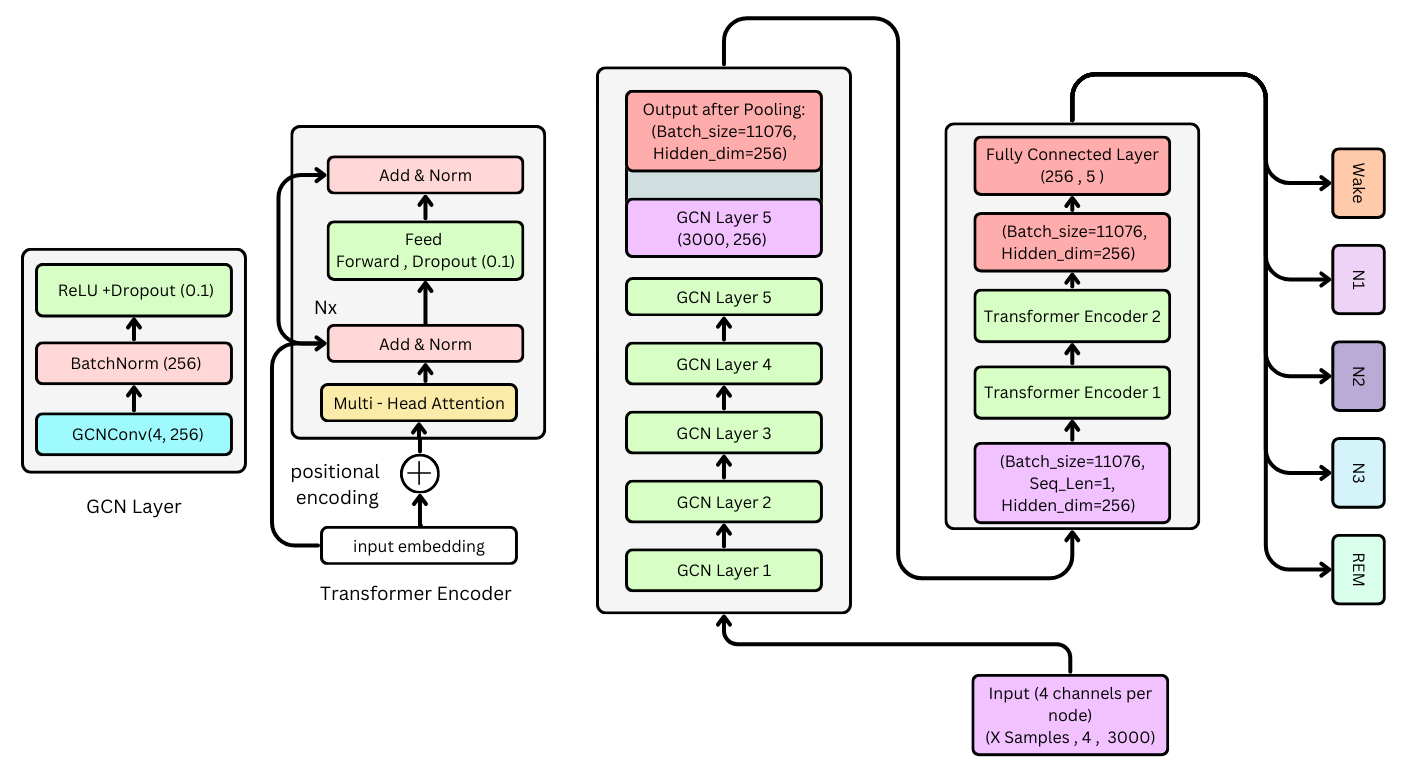
\includegraphics[width=1\linewidth]{img/Architechture.png}
    \caption{Proposed Architecture of GCN-Transformer Hybrid Approach}
    \label{fig:enter-label}
\end{figure}

\subsection{Input Data and Preprocessing}

We use EEG data represented as graph-structured inputs. Each sample contains 4 EEG channels recorded at 3000 frequency points. The dataset dimensions are:
\begin{itemize}
    \item \textbf{X\_all}: (11076, 4, 3000) - Samples, Channels, Frequency Points
    \item \textbf{Y\_all}: (11076,) - Labels for sleep stages
    \item Converted to PyTorch tensors:
    \begin{itemize}
        \item \textbf{X\_tensor}: torch.Size([11076, 4, 3000])
        \item \textbf{Y\_tensor}: torch.Size([11076])
    \end{itemize}
\end{itemize}

\subsubsection{Sleep Stage Mapping}

The sleep stages are mapped as follows:

\begin{table}[h]
\centering
\caption{Mapping of Original Sleep Stages to Labels}
\[
\begin{array}{|c|c|}
\hline
\textbf{Original Stage} & \textbf{Mapped Label} \\
\hline
\text{Sleep stage W} & 0 \\
\text{Sleep stage 1} & 1 \\
\text{Sleep stage 2} & 2 \\
\text{Sleep stage 3} & 3 \\
\text{Sleep stage 4} & 3 \\
\text{Sleep stage R} & 4 \\
\hline
\end{array}
\]
\label{tab:sleep_stage_mapping}
\end{table}


\subsubsection{Channel Selection}

The following EEG channels are selected for analysis: EEG Fpz-Cz, EEG Pz-Oz, EMG submental, and EOG horizontal.

\subsubsection{Preprocessing}

\textbf{Epoch Segmentation:}  
The EEG signals are segmented into 30-second epochs. Each epoch contains 3000 samples per channel, resulting in the final shape of the data as:

\[
\text{Final Data Shape: } [X, 4, 3000]
\]

\textbf{Band-Pass Filtering:}  
A band-pass filter with a frequency range of 0.3 - 30 Hz is applied to the signals. This removes frequencies outside this range, filtering out high-frequency noise and low-frequency drift.






\subsection{Graph Construction}

We represent each sample as a graph, where nodes correspond to EEG channels and edges represent spatial relationships. The graph is defined as:
\begin{itemize}
    \item \textbf{x}: Node features (shape: [3000, 4]) - EEG signals per channel
    \item \textbf{edge\_index}: Graph connectivity (shape: [2, 12])
    \item \textbf{y}: Sleep stage label for each sample (shape: [1])
\end{itemize}

\subsubsection{Methodology: Graph Dataset Creation}

The graph's adjacency matrix represents the spatial relationship between EEG channels. The edge weights are derived from the following graph adjacency matrix:

\begin{table}[h]
\centering
\caption{Graph Weight Representation}
\[
\begin{array}{|c|c|c|c|c|}
\hline
\textbf{} & \textbf{Fpz-Cz} & \textbf{Pz-Oz} & \textbf{EMG} & \textbf{EOG} \\
\hline
\textbf{Fpz-Cz} & 0 & 0.9 & 0.6 & 0.6 \\
\textbf{Pz-Oz}  & 0.9 & 0 & 0.6 & 0.6 \\
\textbf{EMG}    & 0.6 & 0.6 & 0 & 0.5 \\
\textbf{EOG}    & 0.6 & 0.6 & 0.5 & 0 \\
\hline
\end{array}
\]
\label{tab:correlation_matrix}
\end{table}


This matrix is used to define the weights of the edges between the EEG channels in the graph. The value at position \((i, j)\) indicates the weight of the edge between node \(i\) and node \(j\).

\begin{table}[ht]
\centering
\caption{Dataset shape Information}
\begin{tabular}{|c|c|}
\hline
\textbf{Component} & \textbf{Details} \\
\hline
\textbf{Total Samples} & 11,076 \\
\hline
\textbf{Example Sample Format} & Data(x=[3000, 4], edge index=[2, 12], edge attr=[12], y=[1]) \\
\hline
\textbf{x (Node features)} & EEG signals (shape: [3000, 4]) \\
\hline
\textbf{edge index} & Connectivity between EEG channels (shape: [2, 12]) \\
\hline
\textbf{edge attr} & Weights of edges between EEG channels (shape: [12]) \\
\hline
\textbf{y (Label)} & Sleep stage label for the sample (shape: [1]) \\
\hline
\end{tabular}

\end{table}


\subsubsection{Graph Representation of EEG Channels}
The EEG channels are represented as nodes in the graph, with edges indicating spatial relationships based on the adjacency matrix. The resulting graph structure captures both the spatial dependencies between the channels and the temporal dynamics of the EEG signals.
\begin{figure}[!h]
    \centering
    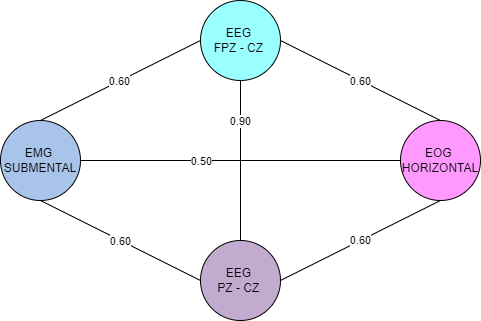
\includegraphics[width=0.5\linewidth]{img/Graph Weightage.png}
    \caption{Graph Weight Visulization}
    \label{fig:enter-label}
\end{figure}






\subsection{GCN Layers for Spatial Feature Extraction}

The GCN module captures spatial dependencies among EEG channels. We employ five Graph Convolutional Network (GCN) layers to learn the connectivity patterns between EEG channels, thereby enhancing feature extraction by leveraging the graph structure of EEG data. The architecture of each GCN layer is described as follows:

\begin{figure}
    \centering
    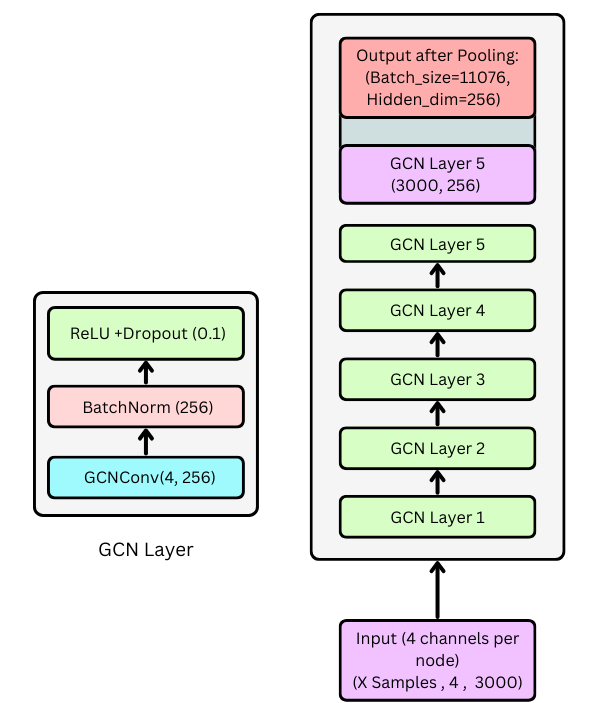
\includegraphics[width=0.7\linewidth]{img/Graph Convolution Neural Network.png}
    \caption{Graph Convolution Neural Network}
    \label{fig:enter-label}
\end{figure}
\begin{table}[ht]
\centering
\caption{GCN Layer Architecture}

\begin{tabular}{|c|c|}
\hline
\textbf{Layer} & \textbf{Operations} \\
\hline
\textbf{GCN Layer 1} & GCNConv(4, 256) $\rightarrow$ BatchNorm(256) $\rightarrow$ ReLU $\rightarrow$ Dropout(0.1) \\
\hline
\textbf{GCN Layer 2 to 5} & GCNConv(256, 256) $\rightarrow$ BatchNorm(256) $\rightarrow$ ReLU $\rightarrow$ Dropout(0.1) \\
\hline
\end{tabular}
\end{table}


 

 

The GCN layers work by taking the input features, which are of shape (4, 256) after the first layer, then passing them through a \textbf{Batch Normalization} layer with 256 output channels. The output is then activated using the \textbf{ReLU} activation function, formulated as:

\[
\text{ReLU}(x) = \max(0, x)
\]


This is followed by \textbf{Dropout}(0.1) for regularization, helping to avoid overfitting by randomly setting 10\% of the input units to zero.

After passing through all five GCN layers, the final output tensor has a shape of \( (3000, 256) \), representing 3000 frequency points with a 256-dimensional feature representation for each frequency point across all EEG channels.

To obtain a graph-level representation, we apply \textbf{global mean pooling} across nodes, which reduces the output to a \( \text{(Batch\_size}=11076, 256) \) tensor. This means that each sample is represented by a single 256-dimensional feature vector. The hidden dimension in this final layer is 256, which captures the most relevant features of the input data.



 

\subsection{Transformer Encoder for Temporal Dependencies}

\begin{table}[!h]
\centering
\caption{Transformer Encoder Overview}

\begin{tabular}{|c|c|}
\hline
\textbf{Component} & \textbf{Details} \\
\hline
\textbf{Preprocessing} & Expand graph embedding to (Batch\_size, 1, 256) \\
\hline
\textbf{Transformer Encoder} & 2 Transformer Encoder Layers \\
\hline
\textbf{d\_model (Hidden dimension)} & 256 \\
\hline
\textbf{nhead (Number of heads)} & 4 \\
\hline
\textbf{Dropout} & 0.1 \\
\hline
\textbf{batch first} & True \\
\hline
\textbf{Postprocessing} & Squeeze output to (Batch\_size, 256) \\
\hline
\textbf{Fully Connected Layer} & Linear(256 $\rightarrow$ 5) \\
\hline
\textbf{Output} & Logits for 5-class classification \\
\hline
\end{tabular}
\end{table}

\begin{figure}[!h]
    \centering
    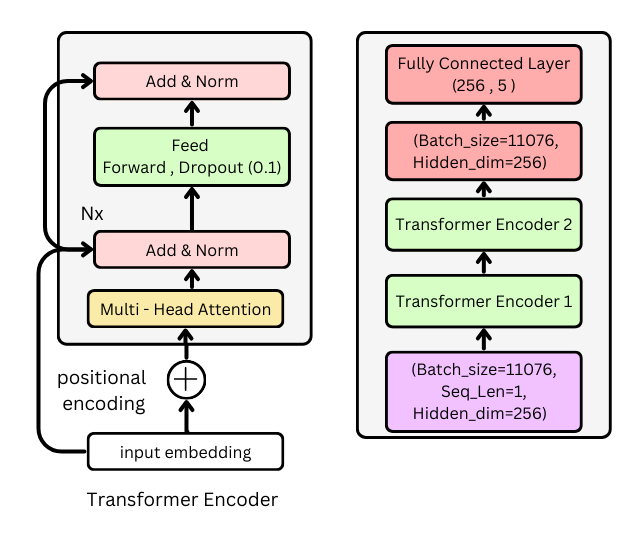
\includegraphics[width=0.7\linewidth]{img/transformer.png}
    \caption{Enter Caption}
    \label{fig:enter-label}
\end{figure}

The Transformer architecture follows the GCN layer pooling shapes. After pooling, the embeddings are passed through the multi-head attention mechanism, followed by Add \& Norm, which normalizes the output. This is then followed by a feed-forward layer, dropout with a 0.1 probability, and another Add \& Norm. The input embeddings are connected in parallel with the Add \& Norm. Positional encoding is applied during input to account for the temporal order of the sequence. The batch size is set to 1, with a sequence length of 1 and a hidden dimension of 256. The input passes through two Transformer Encoder layers, followed by a fully connected linear layer with a transformation from 256 to 5, which outputs the logits for 5-class classification. The final output is obtained using the softmax function, represented by:

\[
\text{Softmax}(z_i) = \frac{e^{z_i}}{\sum_j e^{z_j}}
\]



 
\subsection{Loss Function and Optimization}
We employ Focal Loss to address class imbalance, with parameters:
\begin{itemize}
    \item Gamma ($\gamma$): 3
    \item Label smoothing: 0.1
    \item Class weights computed from the dataset
\end{itemize}

The optimizer and learning rate scheduler are configured as follows:
\begin{itemize}
    \item \textbf{Optimizer}: AdamW (learning rate=0.0003, weight decay=1e-4)
    \item \textbf{Scheduler}: Cosine Annealing Learning Rate Scheduler
\end{itemize}

\subsubsection{Why Focal Loss Instead of Standard Cross-Entropy?}
\textbf{Motivation for Focal Loss:}  
Standard Cross-Entropy treats all samples equally, leading to bias towards majority classes. In imbalanced datasets, minority class predictions get suppressed. Focal Loss dynamically adjusts the loss contribution based on prediction confidence. It reduces the importance of well-classified samples and focuses more on hard-to-classify ones.

\textbf{Key Features of Focal Loss:}
\begin{itemize}
    \item Introduces a focusing parameter $\gamma$ to adjust class weighting.
    \item Includes class weighting factor $\alpha$ to handle imbalance.
    \item Works well for highly imbalanced datasets in classification tasks.
\end{itemize}

\subsubsection{Focal Loss Formulation}
The Focal Loss is formulated as follows:

\[
FL(p_t) = -\alpha (1 - p_t)^{\gamma} \log(p_t)
\]
where:
\begin{itemize}
    \item $p_t$ is the predicted probability for the target class.
    \item $\alpha$ is the weighting factor for class imbalance.
    \item $\gamma$ is the focusing parameter (higher values focus more on hard examples).
\end{itemize}

\subsubsection{Implementation Details}
\textbf{Label Smoothing:} Label smoothing is applied to prevent the log(0) issue by adding a small constant $\epsilon$:

\[
y_{\text{smooth}} = y(1 - \epsilon) + \frac{\epsilon}{C}
\]
where $C$ is the number of classes.

The PyTorch-based computation for Focal Loss with label smoothing becomes:

\[
L = \alpha (1 - p)^{\gamma} (-y_{\text{smooth}} \log p)
\]

\subsubsection{Why Use a Learning Rate Scheduler?}
\textbf{Importance of Learning Rate Scheduling:} The learning rate is crucial for training deep models efficiently. A high learning rate can lead to divergence, while a low one may cause slow convergence. Adaptive learning rate schedules help balance stability and speed.

\textbf{Why CosineAnnealingLR?} Cosine Annealing smoothly reduces the learning rate following a cosine decay. It starts with a large step size for exploration and gradually fine-tunes. This helps avoid sharp drops in the learning rate, improving generalization.

\subsubsection{Cosine Annealing Learning Rate Decay}
The learning rate decay is governed by the formula:

\[
\eta_t = \eta_{\min} + \frac{1}{2} (\eta_{\max} - \eta_{\min}) \left( 1 + \cos\left( \frac{T_{\text{cur}}}{T_{\text{max}}} \pi \right) \right)
\]
where:
\begin{itemize}
    \item $\eta_t$ is the learning rate at epoch $t$.
    \item $\eta_{\max}$ and $\eta_{\min}$ are the max/min learning rates.
    \item $T_{\text{cur}}$ is the current epoch.
    \item $T_{\text{max}}$ is the total number of epochs.
\end{itemize}

\textbf{Key Benefits:}
\begin{itemize}
    \item Encourages large updates early in training.
    \item Smoothly transitions into finer updates as training progresses.
    \item Helps the model avoid getting stuck in poor local minima.
\end{itemize}

\subsubsection{Training Methodology: Overview}
\textbf{SleepTrainer Class: Key Features:}
\begin{itemize}
    \item Handles model training, validation, and optimization.
    \item Uses Focal Loss to address class imbalance.
    \item Applies CosineAnnealingLR scheduler for smooth learning rate decay.
\end{itemize}

\textbf{Training Process:}
\begin{itemize}
    \item Compute class weights for imbalanced data.
    \item Iterate through training batches, compute loss, and update weights.
    \item Validate model performance on a separate validation set.
    \item Adjust learning rate dynamically using a scheduler.
\end{itemize}

\subsubsection{Training Methodology: Hyperparameters}
\textbf{Key Hyperparameters:}
\begin{itemize}
    \item Batch Size: 32
    \item Learning Rate: 0.0003
    \item Weight Decay: 1e-4
    \item Epochs: 20
    \item Optimizer: AdamW
    \item Learning Rate Scheduler: CosineAnnealingLR
\end{itemize}
Gradually reduces learning rate over time for smooth convergence, helping prevent sudden drops in performance.

\subsubsection{Training Methodology: Handling Class Imbalance}
\textbf{Why Compute Class Weights?}  
EEG sleep data is imbalanced, with some sleep stages appearing more frequently. Without weighting, the model may favor majority classes. Weights ensure rare classes contribute more to the loss.

\textbf{Class Weight Computation:}
The class weight for class $c$ is computed as:

\[
w_c = \left( \frac{\text{Total Samples}}{\text{Class Count} + 1} \right)^{0.5}
\]
where:
\begin{itemize}
    \item $w_c$ is the computed weight for class $c$.
    \item Smaller classes receive higher weights.
\end{itemize}

These weights are applied to the Focal Loss during training.






 


        
 	\chapter[Results and Discussion]
    {Results and Discussion}


\subsection{Testing Data Distribution Analysis}

\textbf{Why Ensure Balanced Testing Data?}
\begin{itemize}
    \item Prevents bias toward majority classes.
    \item Ensures the model’s performance is fairly evaluated.
    \item Helps achieve reliable generalization across all sleep stages.
\end{itemize}

The figure below shows the normalized class distribution during testing. Each class maintains an equalized density, avoiding class imbalance. This confirms that the model’s evaluation is not biased toward any specific sleep stage.

\textbf{Sampling Density Plot Showing Balanced Class Distribution:}
\begin{figure}[h!]
    \centering
    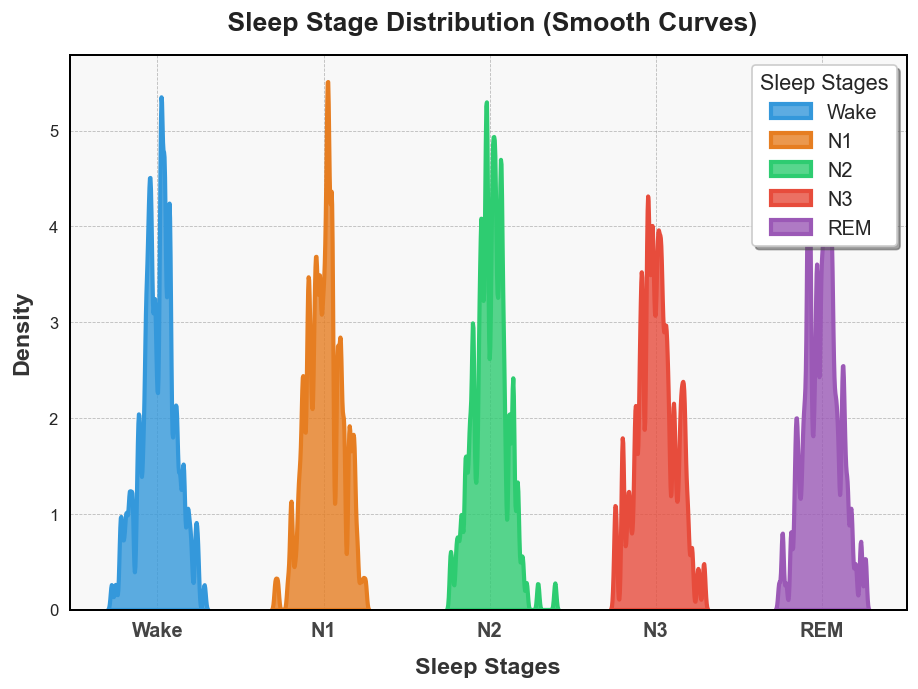
\includegraphics[width=0.8\textwidth]{img/sample distribution plot pdf.png}
    \caption{Balanced class distribution across the test set.}
\end{figure}

\subsection{Model Performance: Training vs Testing}

Figures below demonstrate the accuracy and loss curves during training and testing, providing a clear visual comparison of model performance:

\begin{figure}[h!]
    \centering
    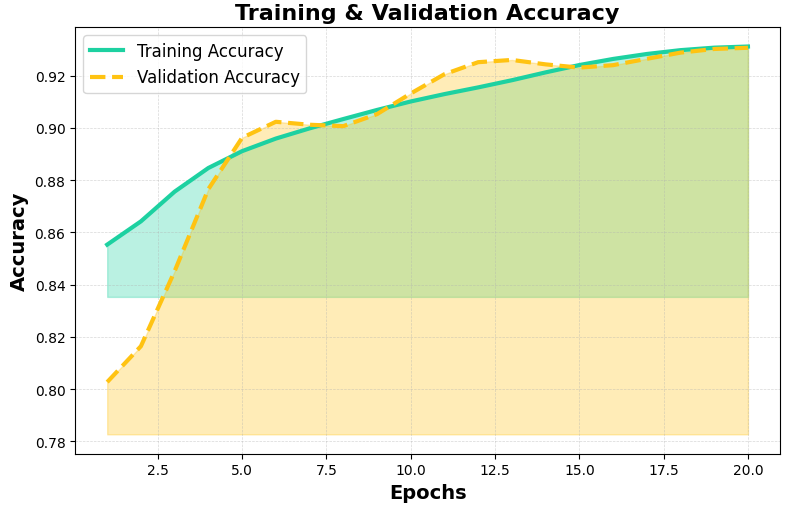
\includegraphics[width=0.8\textwidth]{img/accuracy plot.png}
    \caption{Accuracy Curve: Training vs Testing.}
\end{figure}

\begin{figure}[h!]
    \centering
    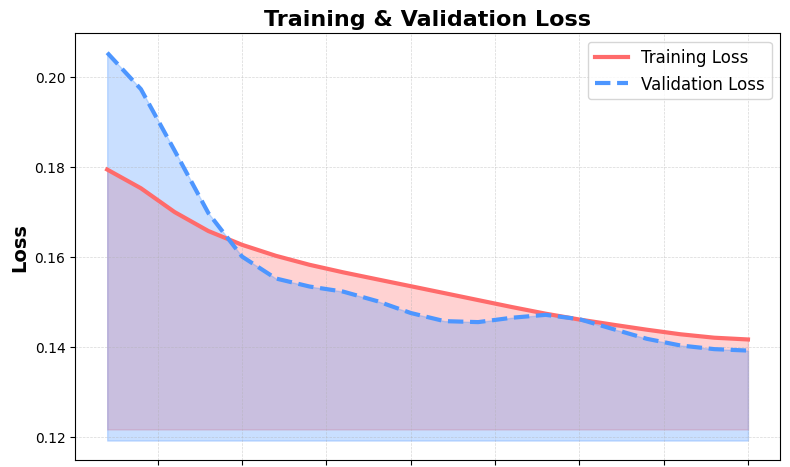
\includegraphics[width=0.8\textwidth]{img/loss plot.png}
    \caption{Loss Curve: Training vs Testing.}
\end{figure}

\subsection{Model Evaluation: Confusion Matrix}

Performance metrics are calculated to ensure a comprehensive evaluation of the model's performance across all classes. We use precision, recall, and F1-score to assess the model:

\[
\text{Precision} = \frac{TP}{TP + FP}
\]
\[
\text{Recall} = \frac{TP}{TP + FN}
\]
\[
\text{F1-Score} = \frac{2 \times \text{Precision} \times \text{Recall}}{\text{Precision} + \text{Recall}}
\]

These metrics ensure a balanced evaluation of model performance across all sleep stages.

\begin{figure}[h!]
    \centering
    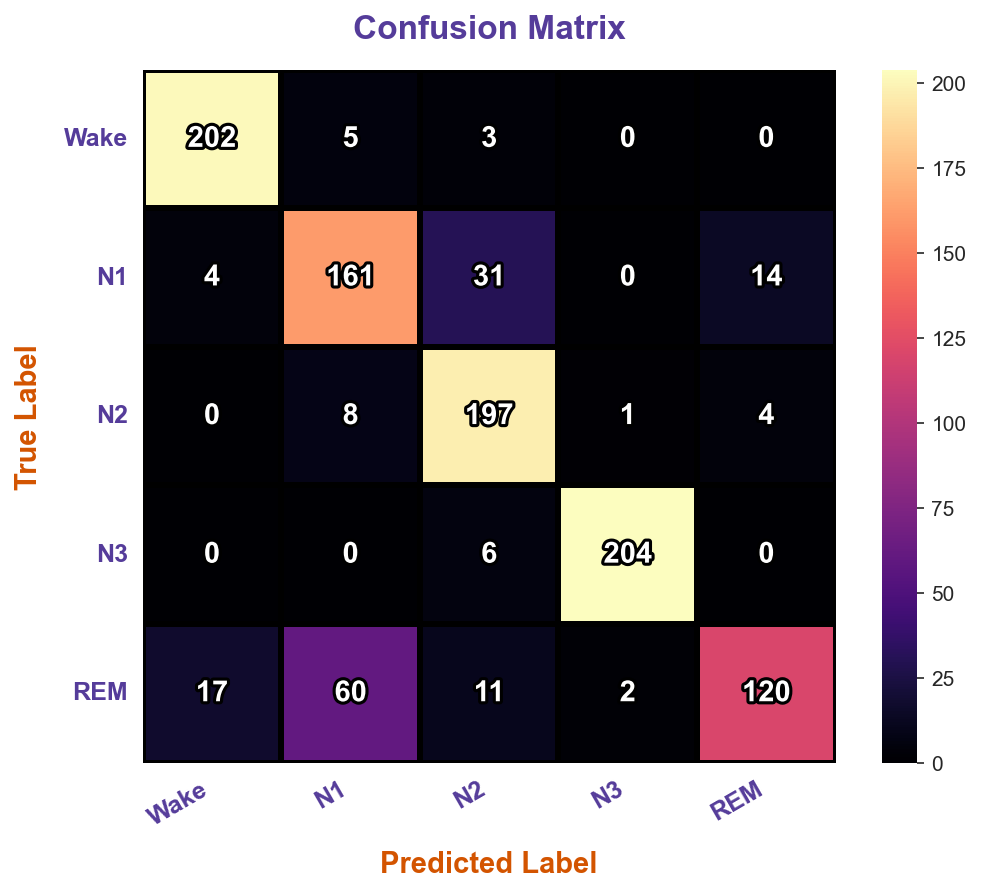
\includegraphics[width=0.8\textwidth]{img/confusion matrix samples.png}
    \caption{Confusion Matrix showing model performance across sleep stages.}
\end{figure}

\subsection{Gradient Analysis: Training Progression}

Understanding model training dynamics:

\textbf{Early Training (Epochs 0-5):} High loss with accuracy starting to improve.  
\textbf{Mid Training (Epochs 5-15):} Loss steadily decreases with stable gradient flow.  
\textbf{Late Training (Epochs 15-20):} Accuracy plateaus with no severe overfitting.

\textbf{Conclusion:} The training process remains stable, with no vanishing or exploding gradients.

\begin{figure}[h!]
    \centering
    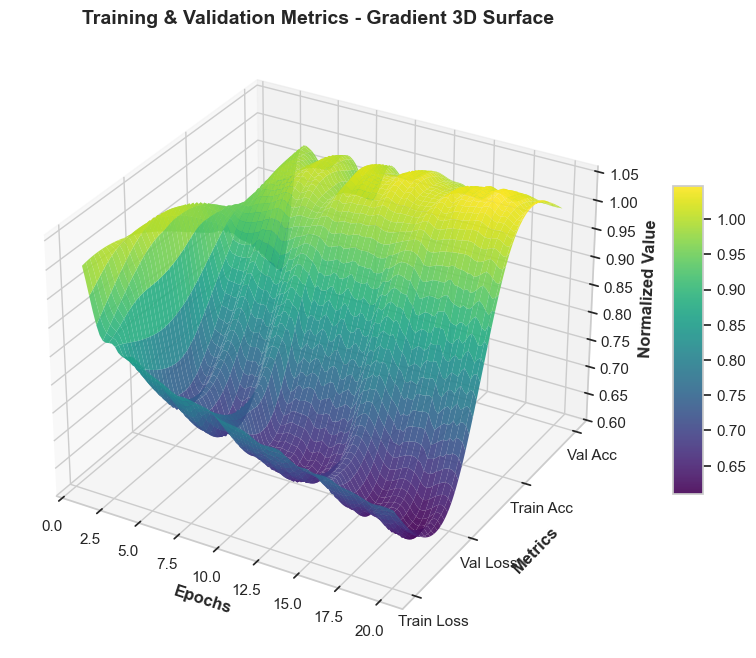
\includegraphics[width=0.8\textwidth]{img/3d gradient.png}
    \caption{Gradient 3D Surface: Training vs Validation Metrics.}
\end{figure}

\subsection{Performance Metrics: Precision, Recall, F1-Score}

Evaluating model performance across all classes using key metrics:

\begin{figure}[h!]
    \centering
    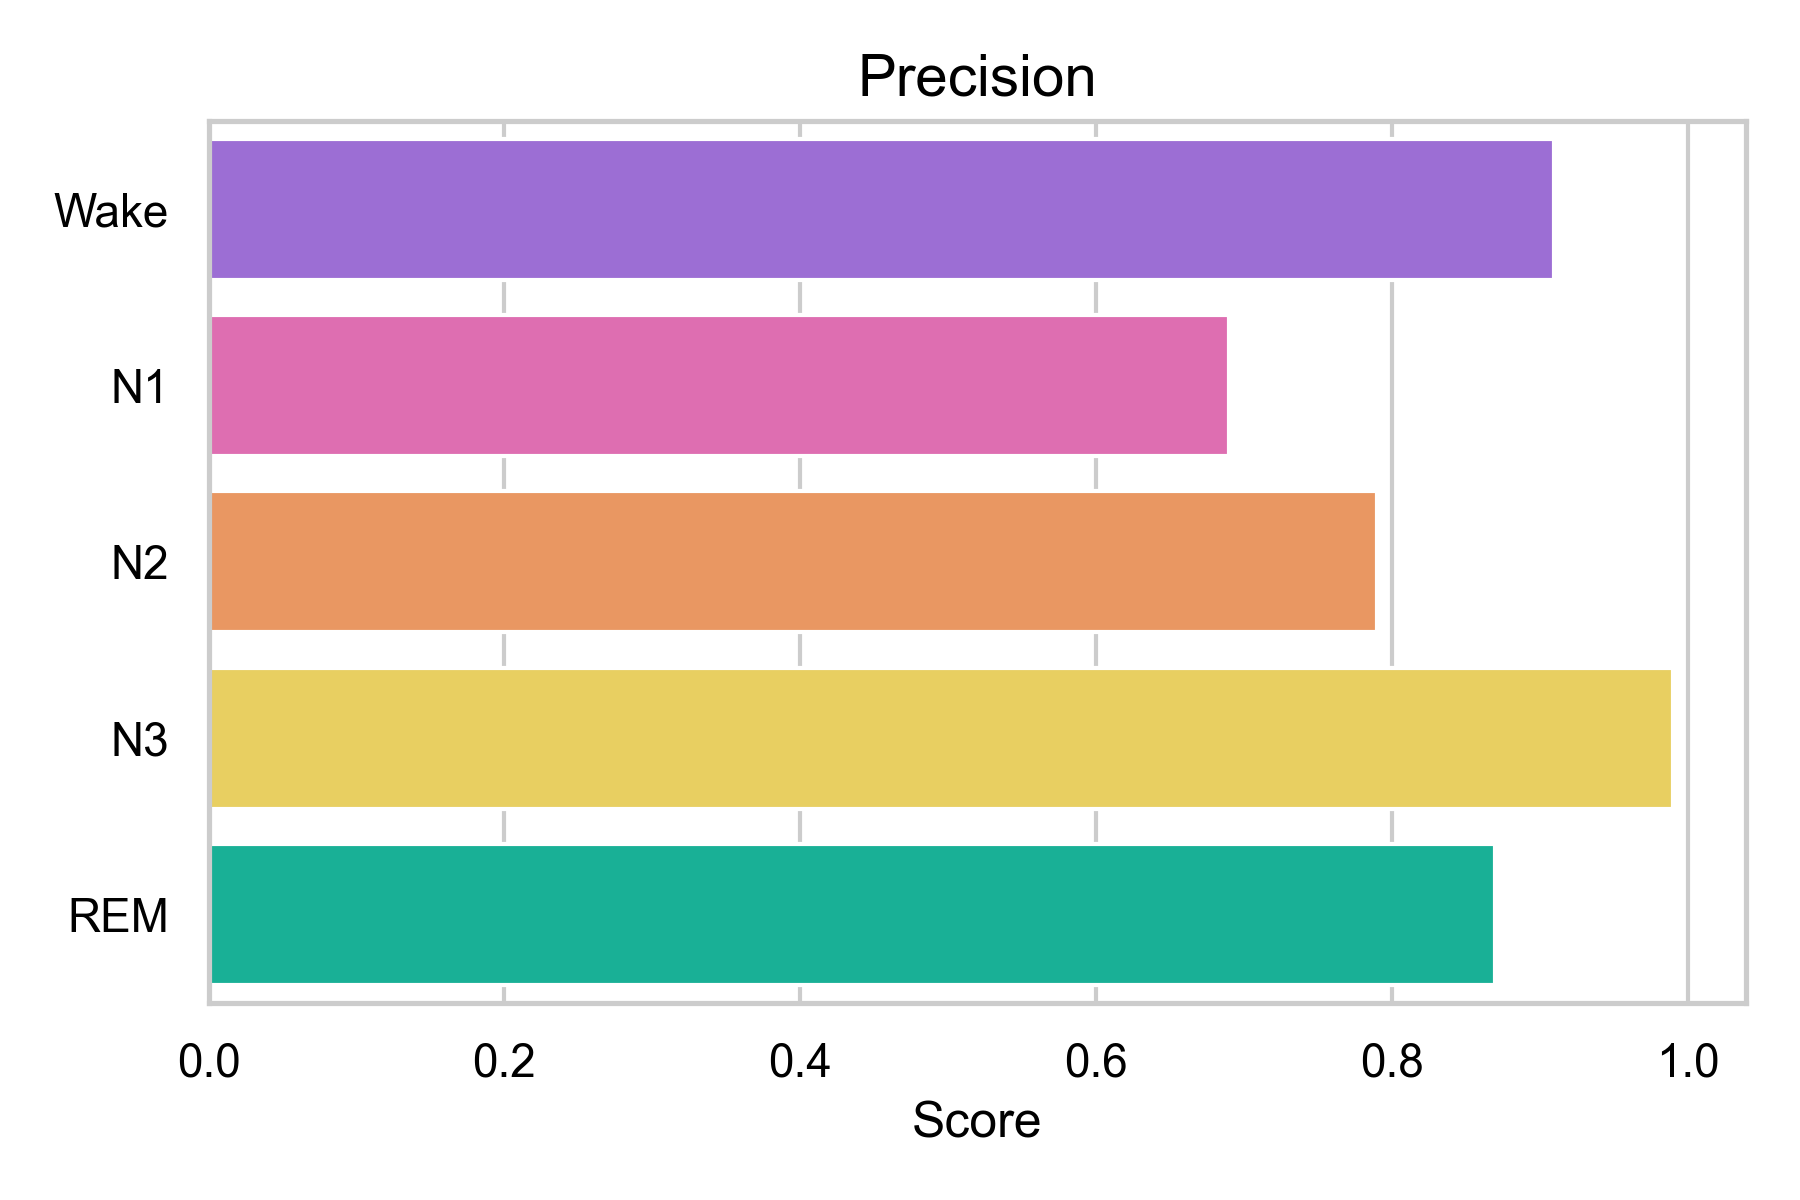
\includegraphics[width=0.8\textwidth]{img/precision_plot.png}
    \caption{Precision Scores per Class.}
\end{figure}

\begin{figure}[h!]
    \centering
    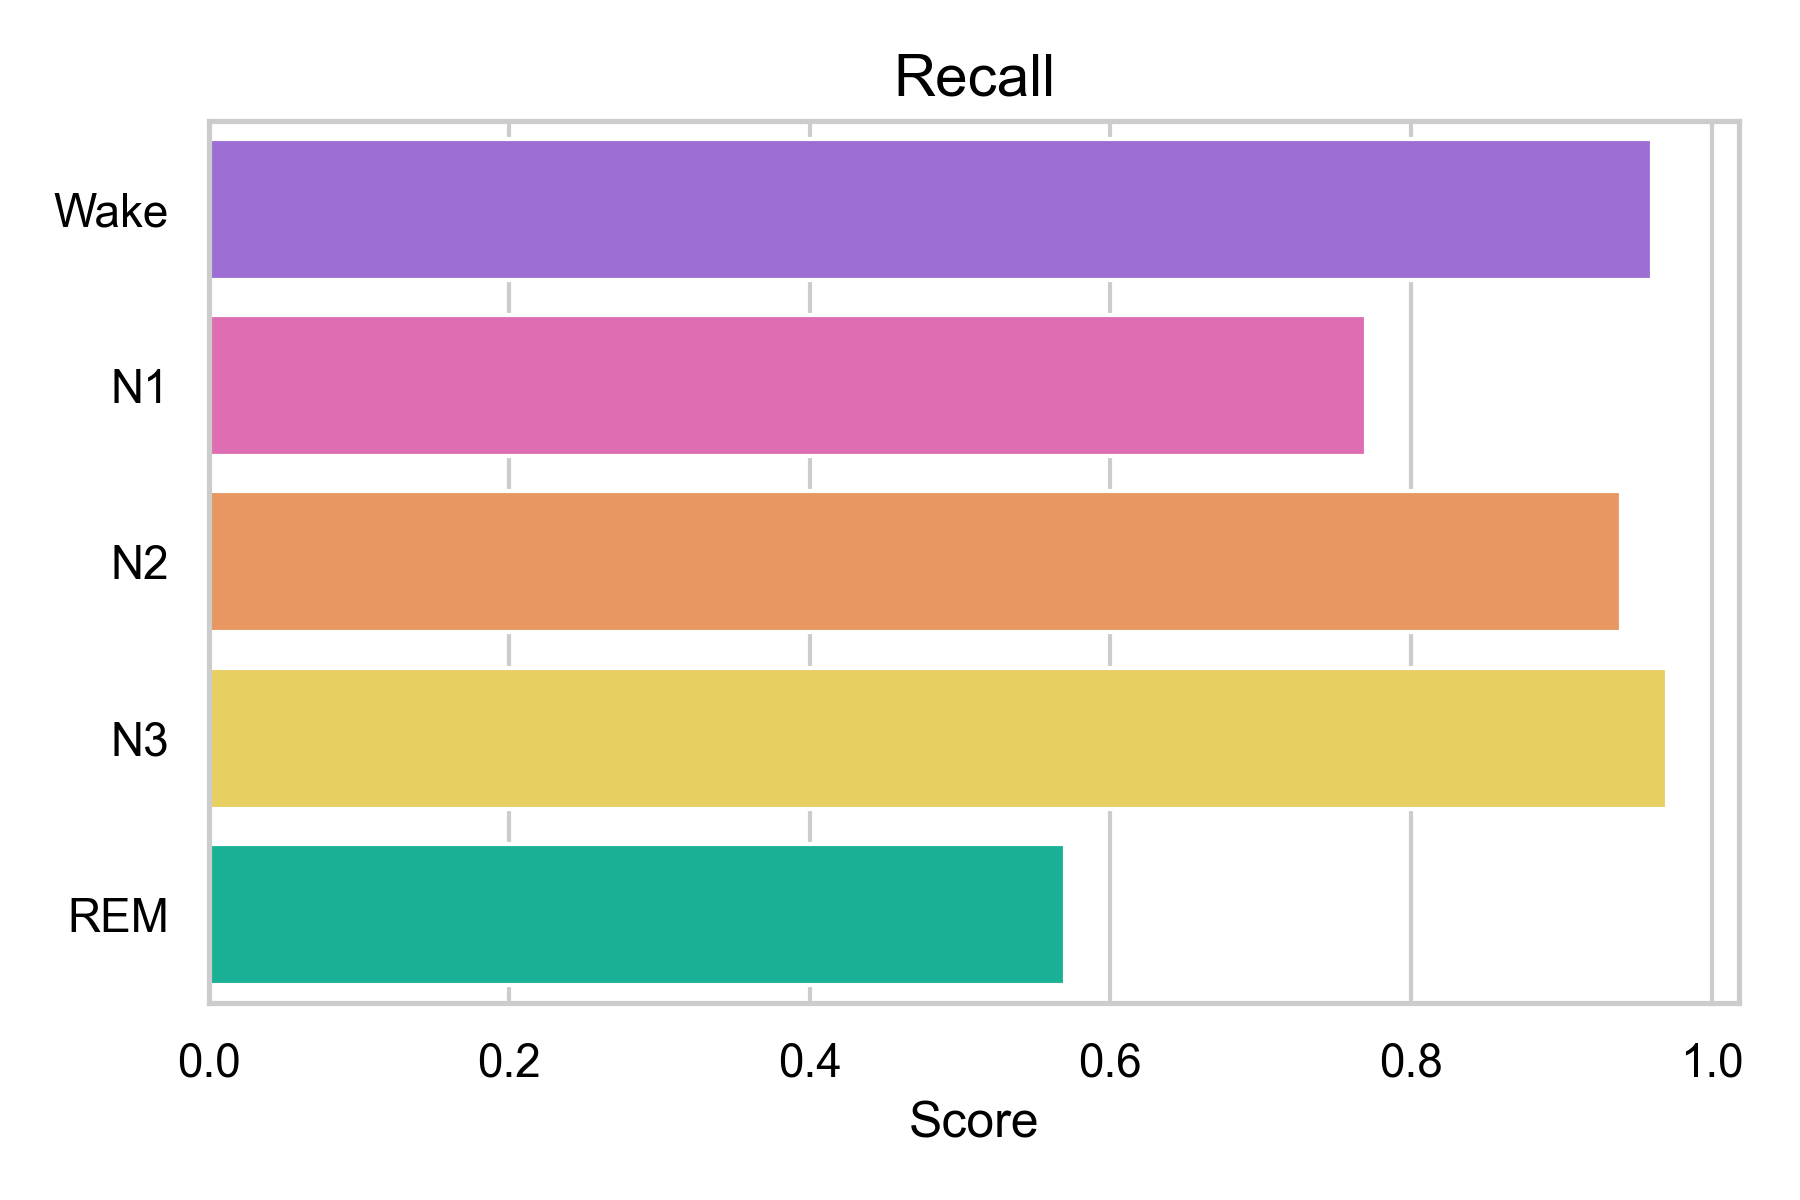
\includegraphics[width=0.8\textwidth]{img/recall_plot.png}
    \caption{Recall Scores per Class.}
\end{figure}

\begin{figure}[h!]
    \centering
    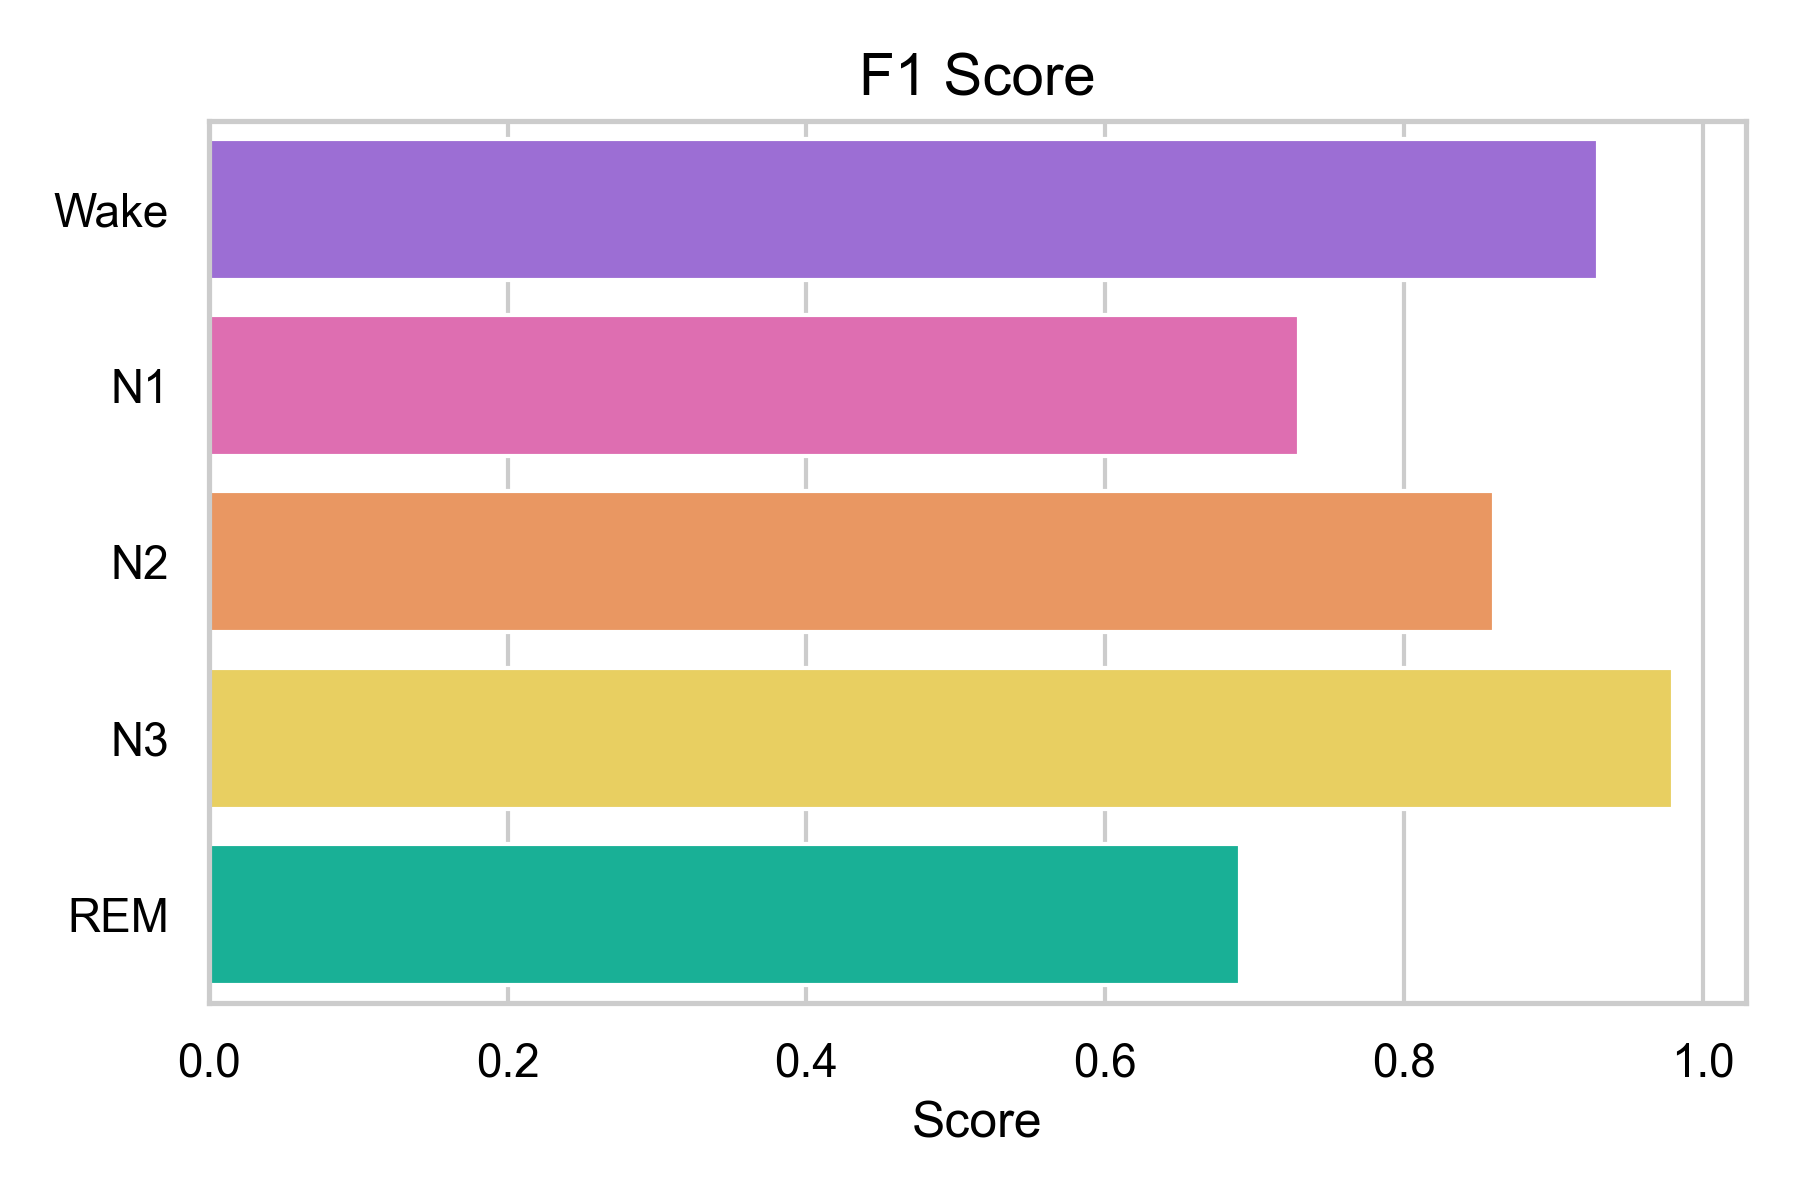
\includegraphics[width=0.8\textwidth]{img/f1_score_plot.png}
    \caption{F1 Scores per Class.}
\end{figure}

\subsection{Feature Importance Analysis with LIME}

Understanding the contribution of different channels to model predictions, we used LIME (Local Interpretable Model-agnostic Explanations) to analyze feature importance. The analysis showed that the \textbf{EMG submental} and \textbf{EEG Pz-Oz} channels contribute the most to predictions, while the \textbf{EOG horizontal} channel has minimal importance, indicating lower relevance for classification.

This insight helps optimize feature selection and improve model efficiency.

\begin{figure}[h!]
    \centering
    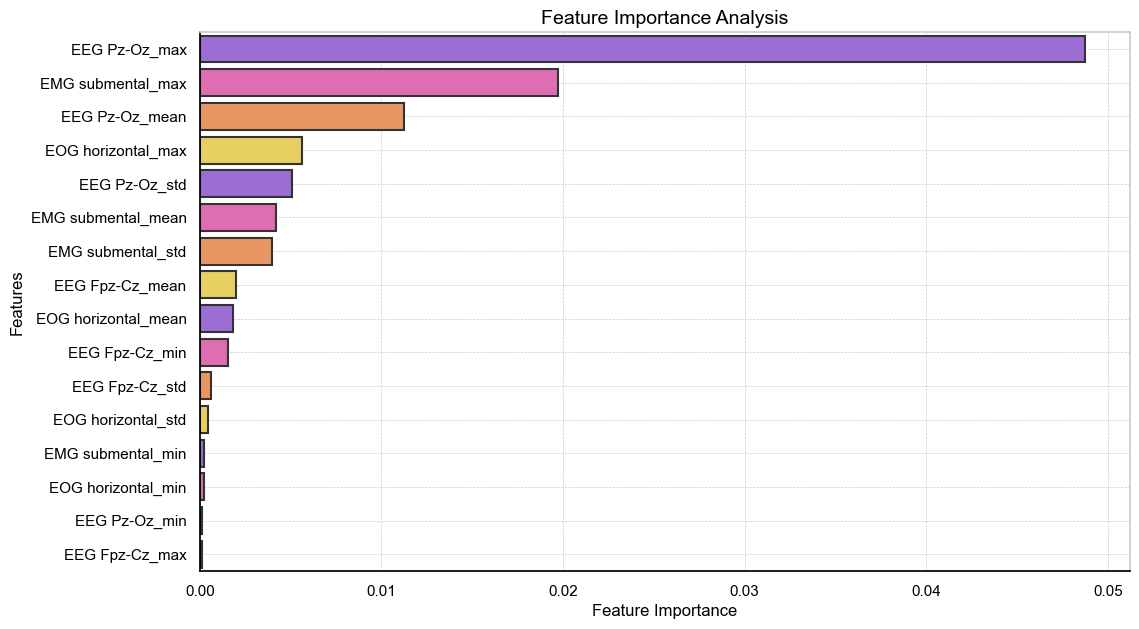
\includegraphics[width=0.8\textwidth]{img/feature importance chanels analysis.png}
    \caption{Feature Importance Analysis for 4 Channels.}
\end{figure}

	
	\chapter[Conclusion]{Conclusion}
	\pagestyle{plain}
 \section{Discussion}

\subsection{Principal Contributions}
This study proposes a novel graph-based representation for sleep EEG data, integrating a hybrid GCN-Transformer architecture to improve the classification of sleep stages. By effectively capturing both spatial and temporal dependencies, our model outperforms traditional deep learning approaches in terms of accuracy and robustness. The incorporation of graph structures, combined with attention mechanisms, facilitates a more nuanced understanding of sleep dynamics.

\subsection{Distinctive Aspects of Our Approach}
Conventional methods such as CNNs primarily emphasize spatial features, whereas RNNs address temporal dynamics but are limited in handling long-range dependencies. Our model bridges this gap by combining the spatial modeling capabilities of Graph Convolutional Networks (GCNs) with the sequence modeling strengths of Transformers. Moreover, the use of Focal Loss and Label Smoothing addresses class imbalance effectively. The explainability component of our framework, supported by XAI techniques, identifies key EEG channels that influence sleep stage transitions, enhancing interpretability and clinical relevance.

\subsection{Performance Highlights}
Several components contribute to the model’s success. The graph-based representation enables the retention of spatial relationships across EEG nodes, promoting more effective learning of brain activity patterns. The fusion of GCN and Transformer modules allows the network to model complex spatial-temporal interactions, yielding highly accurate sleep stage predictions. Techniques for mitigating class imbalance—such as Focal Loss and Label Smoothing—enhance reliability, especially in underrepresented stages. Additionally, explainability features provide actionable insights into the neural correlates of sleep, supporting broader medical and neuroscientific applications.

\subsection{Limitations and Future Directions}
Despite its strengths, the proposed method has notable limitations. The combined GCN-Transformer model incurs higher computational costs compared to lighter architectures like CNNs or LSTMs, which may restrict deployment in resource-constrained environments. The Sleep-EDF dataset, although widely used, includes a limited sample of subjects, potentially affecting generalizability. Furthermore, while acceleration via Apple M1 and Metal APIs improves efficiency, larger models would benefit from more powerful hardware such as GPUs or TPUs. Future work may explore more scalable architectures and validate the approach on larger, more diverse datasets.

\section{Conclusion}

The proposed SleepGCN-Transformer architecture demonstrates superior performance in sleep stage classification, achieving 93.12\% training accuracy and 93.04\% validation accuracy. By integrating GCNs to model spatial interdependencies and Transformers to extract temporal patterns, the model effectively captures the complexity of sleep physiology. The application of Focal Loss contributes to robust handling of class imbalance, improving classification across all stages. Feature importance analysis indicates that EMG and the EEG Pz-Oz channel play a critical role in prediction. This approach not only improves predictive performance but also enhances interpretability, laying a foundation for future work in explainable and clinically applicable sleep analysis tools.


\chapter [Reference] {Reference}
		\pagestyle{plain}
	 \begin{thebibliography}{99}
	
	\bibitem{han2024classification}
	H.~Han et~al., ``Classification and automatic scoring of arousal intensity during sleep stages using machine learning,'' \emph{Scientific Reports}, vol.~14, no.~1, Dec. 2024, doi: \href{https://doi.org/10.1038/s41598-023-50653-9}{10.1038/s41598-023-50653-9}.
	
	\bibitem{tsinalis2016automatic}
	O.~Tsinalis et~al., ``Automatic Sleep Stage Scoring Using Time-Frequency Analysis and Stacked Sparse Autoencoders,'' \emph{Annals of Biomedical Engineering}, vol.~44, no.~5, May 2016, doi: \href{https://doi.org/10.1007/s10439-015-1444-y}{10.1007/s10439-015-1444-y}.
	
	\bibitem{krakovska2011automatic}
	A.~Krakovská and K.~Mezeiová, ``Automatic sleep scoring: A search for an optimal combination of measures,'' \emph{Artificial Intelligence in Medicine}, vol.~53, no.~1, Sep. 2011, doi: \href{https://doi.org/10.1016/j.artmed.2011.06.004}{10.1016/j.artmed.2011.06.004}.
	
	\bibitem{biswal2018expert}
	S.~Biswal et~al., ``Expert-level sleep scoring with deep neural networks,'' \emph{Journal of the American Medical Informatics Association}, vol.~25, no.~12, Dec. 2018, doi: \href{https://doi.org/10.1093/jamia/ocy131}{10.1093/jamia/ocy131}.
	
	\bibitem{ronzhina2012sleep}
	M.~Ronzhina et~al., ``Sleep scoring using artificial neural networks,'' \emph{Sleep Medicine Reviews}, vol.~16, no.~3, Jun. 2012, doi: \href{https://doi.org/10.1016/j.smrv.2011.06.003}{10.1016/j.smrv.2011.06.003}.
	
	\bibitem{alsolai2022systematic}
	H.~Alsolai et~al., ``A Systematic Review of Literature on Automated Sleep Scoring,'' \emph{IEEE Access}, vol.~10, pp.~79419--79443, 2022, doi: \href{https://doi.org/10.1109/ACCESS.2022.3194145}{10.1109/ACCESS.2022.3194145}.
	
	\bibitem{fiorillo2019automated}
	L.~Fiorillo et~al., ``Automated sleep scoring: A review of the latest approaches,'' \emph{Sleep Medicine Reviews}, vol.~48, Dec. 2019, doi: \href{https://doi.org/10.1016/j.smrv.2019.07.007}{10.1016/j.smrv.2019.07.007}.
	
	\bibitem{faust2019review}
	O.~Faust et~al., ``A review of automated sleep stage scoring based on physiological signals for the new millennia,'' \emph{Computer Methods and Programs in Biomedicine}, vol.~176, Jul. 2019, doi: \href{https://doi.org/10.1016/j.cmpb.2019.04.032}{10.1016/j.cmpb.2019.04.032}.
	
	\bibitem{chriskos2021review}
	P.~Chriskos et~al., ``A review on current trends in automatic sleep staging through bio-signal recordings and future challenges,'' \emph{Sleep Medicine Reviews}, vol.~55, Feb. 2021, doi: \href{https://doi.org/10.1016/j.smrv.2020.101377}{10.1016/j.smrv.2020.101377}.
	
	\bibitem{phan2022sleeptransformer}
	H.~Phan, K.~B. Mikkelsen, O.~Y. Chen, P.~Koch, A.~Mertins, and M.~De~Vos, ``SleepTransformer: Automatic Sleep Staging with Interpretability and Uncertainty Quantification,'' \emph{IEEE Transactions on Biomedical Engineering}, 2022.
	
	

	
	\bibitem{han2024classification}
	H.~Han et~al., ``Classification and automatic scoring of arousal intensity during sleep stages using machine learning,'' \emph{Scientific Reports}, vol.~14, no.~1, Dec. 2024.
	
	\bibitem{tsinalis2016automatic}
	O.~Tsinalis et~al., ``Automatic Sleep Stage Scoring Using Time-Frequency Analysis and Stacked Sparse Autoencoders,'' \emph{Annals of Biomedical Engineering}, vol.~44, no.~5, May 2016.
	
	\bibitem{krakovska2011automatic}
	A.~Krakovská and K.~Mezeiová, ``Automatic sleep scoring: A search for an optimal combination of measures,'' \emph{Artificial Intelligence in Medicine}, vol.~53, no.~1, Sep. 2011.
	
	\bibitem{biswal2018expert}
	S.~Biswal et~al., ``Expert-level sleep scoring with deep neural networks,'' \emph{JAMIA}, vol.~25, no.~12, Dec. 2018.
	
	\bibitem{ronzhina2012sleep}
	M.~Ronzhina et~al., ``Sleep scoring using artificial neural networks,'' \emph{Sleep Medicine Reviews}, vol.~16, no.~3, Jun. 2012.
	
	\bibitem{alsolai2022systematic}
	H.~Alsolai et~al., ``A Systematic Review of Literature on Automated Sleep Scoring,'' \emph{IEEE Access}, vol.~10, 2022.
	
	\bibitem{fiorillo2019automated}
	L.~Fiorillo et~al., ``Automated sleep scoring: A review of the latest approaches,'' \emph{Sleep Medicine Reviews}, vol.~48, Dec. 2019.
	
	\bibitem{faust2019review}
	O.~Faust et~al., ``A review of automated sleep stage scoring based on physiological signals for the new millennia,'' \emph{Computer Methods and Programs in Biomedicine}, vol.~176, Jul. 2019.
	
	\bibitem{chriskos2021review}
	P.~Chriskos et~al., ``A review on current trends in automatic sleep staging through bio-signal recordings and future challenges,'' \emph{Sleep Medicine Reviews}, vol.~55, Feb. 2021.
	
	\bibitem{phan2022sleeptransformer}
	H.~Phan et~al., ``SleepTransformer: Automatic Sleep Staging with Interpretability and Uncertainty Quantification,'' \emph{IEEE Transactions on Biomedical Engineering}, 2022.
	
	\bibitem{dai2023multichannelsleepnet}
	Y.~Dai et~al., ``MultiChannelSleepNet: A Transformer-Based Model for Automatic Sleep Stage Classification With PSG,'' \emph{IEEE J. Biomed. Health Inform.}, 2023.
	
	\bibitem{guo2024flexsleeptransformer}
	Y.~Guo, M.~Nowakowski, and W.~Dai, ``FlexSleepTransformer: A Transformer-Based Sleep Staging Model with Flexible Input Channel Configurations,'' \emph{Scientific Reports}, 2024.
	
	\bibitem{yao2022cnntransformer}
	Z.~Yao and X.~Liu, ``A CNN-Transformer Deep Learning Model for Real-time Sleep Stage Classification in an Energy-Constrained Wireless Device,'' \emph{medRxiv}, 2022.
	
	\bibitem{supratak2017deepsleepnet}
	A.~Supratak et~al., ``DeepSleepNet: A Model for Automatic Sleep Stage Scoring Based on Raw Single-Channel EEG,'' \emph{IEEE Trans. Neural Syst. Rehabil. Eng.}, vol.~25, no.~11, pp.~1998--2008, 2017.
	
	\bibitem{eldele2021attnsleep}
	E.~Eldele et~al., ``AttnSleep: An Attention-Based Deep Learning Approach for Sleep Stage Classification With Single-Channel EEG,'' \emph{IEEE Trans. Neural Syst. Rehabil. Eng.}, 2021.
	
	\bibitem{ji2022jkstgcn}
	X.~Ji, Y.~Li, and P.~Wen, ``Jumping Knowledge-Based Spatial-Temporal Graph Convolutional Networks for Automatic Sleep Stage Classification,'' \emph{IEEE Trans. Neural Syst. Rehabil. Eng.}, 2022.
	
	\bibitem{mousavi2019sleepeegnet}
	S.~Mousavi, F.~Afghah, and U.~R. Acharya, ``SleepEEGNet: Automated Sleep Stage Scoring With Sequence-to-Sequence Deep Learning Approach,'' \emph{PLOS ONE}, 2019.
	
	\bibitem{phan2019seqsleepnet}
	H.~Phan et~al., ``SeqSleepNet: End-to-End Hierarchical Recurrent Neural Network for Sequence-to-Sequence Automatic Sleep Staging,'' \emph{IEEE Trans. Neural Syst. Rehabil. Eng.}, 2019.
	
	\bibitem{zhang2024cnntransformerconvlstm}
	Zhang et~al., ``A CNN-Transformer-ConvLSTM-CRF Hybrid Network for Sleep Stage Classification,'' \emph{IEEE Sensors Journal}, 2024.
	
	\bibitem{liu2024review}
	Liu et~al., ``Automatic Sleep Stage Classification Using Deep Learning: Signals, Data Representation, and Neural Networks,'' \emph{Artificial Intelligence Review}, 2024.
	
	\bibitem{ctdal2022}
	CT-DAL, ``Convolutional Transformer with Domain Adversarial Learning for Multi-Channel Sleep Stage Classification,'' \emph{Available on Semantic Scholar}, 2022.
	
	\bibitem{pei2022hybrid}
	W.~Pei, Y.~Li, S.~Siuly, and P.~Wen, ``A Hybrid Deep Learning Scheme for Multi-Channel Sleep Stage Classification,'' \emph{Computers, Materials \& Continua}, 2022.
	
	\bibitem{mostafaei2024crossmodality}
	S.~H. Mostafaei, J.~Tanha, and A.~Sharafkhaneh, ``A Novel Deep Learning Model Based on Transformer and Cross-Modality Attention for Classification of Sleep Stages,'' \emph{Journal of Biomedical Informatics}, 2024.
	
	\bibitem{jeong2024explainablevit}
	Jeong et~al., ``Explainable Vision Transformer for Automatic Visual Sleep Staging,'' \emph{npj Digital Medicine}, 2024.
	
	\bibitem{pei2024mfcc}
	W.~Pei, Y.~Li et~al., ``An Automatic Method Using MFCC Features for Sleep Stage Classification,'' \emph{Biomedical Signal Processing and Control}, 2024.
	
	\bibitem{sors2018cnn}
	A.~Sors et~al., ``A Convolutional Neural Network for Sleep Stage Scoring from Raw Single-Channel EEG,'' \emph{Biomedical Signal Processing and Control}, 2018.
	
	\bibitem{seo2020iitnet}
	H.~Seo et~al., ``Intra- and Inter-Epoch Temporal Context Network (IITNet) Using Sub-Epoch Features for Automatic Sleep Scoring on Raw Single-Channel EEG,'' \emph{Biomedical Signal Processing and Control}, 2020.
	
	\bibitem{biswal2017sleepnet}
	S.~Biswal et~al., ``SLEEPNET: Automated Sleep Staging System via Deep Learning,'' \emph{Journal of the American Medical Informatics Association}, 2017.
	
	\bibitem{phan2018jointcnn}
	H.~Phan et~al., ``Joint Classification and Prediction CNN Framework for Automatic Sleep Stage Classification,'' \emph{IEEE Transactions on Biomedical Engineering}, 2018.
	
\end{thebibliography}






 
        \clearpage\thispagestyle{empty}
\end{document}
